\documentclass[conference]{IEEEtran}

\usepackage[utf8]{inputenc}
\usepackage[T1]{fontenc}
\usepackage[spanish,english]{babel}
\usepackage{graphicx}
\usepackage{amsmath,amssymb}
\usepackage{booktabs}
\usepackage{tabularx}
\usepackage[hidelinks]{hyperref}
\usepackage{float}
\usepackage{xcolor}
\usepackage{colortbl}
\usepackage{cite}
\usepackage{url}
\usepackage{multirow}
\usepackage{makecell}

\definecolor{cellgood}{RGB}{212,237,218}
\definecolor{cellmid}{RGB}{255,243,205}
\definecolor{cellbad}{RGB}{248,215,218}
\newcommand{\cg}[1]{\cellcolor{cellgood}#1}
\newcommand{\cm}[1]{\cellcolor{cellmid}#1}
\newcommand{\cb}[1]{\cellcolor{cellbad}#1}
\newcommand{\na}{\cellcolor{gray!18}N/A}

\graphicspath{{figuras/}}

\title{Segmentaci\'{o}n cl\'{a}sica del tumor realzante en glioma
post-tratamiento sobre BraTS~2024}

\author{%
\IEEEauthorblockN{Abel Albuez, Victoria Acero y Santiago Gil}
\IEEEauthorblockA{Maestr\'{i}a en Ingenier\'{i}a de Sistemas y Computaci\'{o}n\\
Pontificia Universidad Javeriana, Bogot\'{a} D.C., Colombia\\
Procesamiento de Im\'{a}genes M\'{e}dicas, 2026\\
\url{https://github.com/AbelAlbuez/medical-image-processing}}}

\begin{document}
\maketitle

% ═══════════════════════════════════════════
\begin{abstract}
Automatic segmentation of the enhancing tumor subregion in
post-treatment glioma MRI remains an open problem for classical
methods, as the resection cavity and treatment-related changes
drastically alter the intensity patterns these methods rely on.
This work evaluates a fully classical pipeline, implemented with
SimpleITK and without any deep-learning component, on 20~randomly
selected cases from the BraTS~2024~GLI Post-Treatment dataset.
The pipeline applies a preprocessing stage that combines a Wiener
filter, N4 bias-field correction, and percentile normalization,
followed by a rigid-registration demonstration using Mattes mutual
information that achieves a sub-voxel target registration error
of 0.007~mm on average.
For segmentation, four intensity-based methods are evaluated on
contrast-enhanced T1-weighted images---multilevel Otsu
thresholding, region growing, watershed by markers, and
multimodal Gaussian mixture models---whose best union ensemble
reaches a mean Dice of 0.370.
To overcome the structural ceiling of intensity-only approaches,
a gadolinium-specific subtraction map computed as T1-contrast
minus T1-native is introduced, yielding mean values of 0.24
within the enhancing tumor versus 0.04 in healthy tissue.
This map drives two complementary methods: a FastMarching
algorithm that uses it as a propagation-speed function (Dice
0.509 with a centroid seed, 0.286 with automatic seeding), and
variational active contours, among which the Chan--Vese
variational spline achieves the best mean Dice of 0.505 with
automatic seeding and a maximum of 0.860 on the most favorable
individual case.
Results show that intensity-only methods have a structural
ceiling imposed by the shape of the post-surgical enhancing
tumor, while the T1c$-$T1n subtraction map provides a
discriminative signal that enables classical methods to exceed
Dice~0.50 without deep learning.
\end{abstract}

\begin{IEEEkeywords}
BraTS 2024 GLI, tumor realzante, segmentaci\'{o}n cl\'{a}sica,
FastMarching, contornos activos, Chan--Vese, SimpleITK, mapa de
sustracci\'{o}n T1c$-$T1n.
\end{IEEEkeywords}

% ═══════════════════════════════════════════
\section{Introducci\'{o}n}
% ═══════════════════════════════════════════

Los gliomas son los tumores cerebrales primarios m\'{a}s frecuentes
en adultos y su seguimiento por resonancia magn\'{e}tica es
indispensable para evaluar la respuesta al tratamiento y detectar
recurrencia temprana~\cite{louis2021who,mesfin2024gliomas}.
El tumor realzante, definido como el tejido que capta el agente de
contraste gadolinio en secuencias T1 post-contraste, constituye
el marcador imagenol\'{o}gico de actividad tumoral residual m\'{a}s
utilizado y un sustituto habitual de la respuesta
terap\'{e}utica~\cite{bhattacharya2024posttreatment}.
Su delimitaci\'{o}n manual es laboriosa y presenta una variabilidad
inter-observador significativa incluso entre radi\'{o}logos
especializados~\cite{visser2019interobserver}, lo que motiva la
b\'{u}squeda de m\'{e}todos de segmentaci\'{o}n autom\'{a}tica.

El escenario post-tratamiento introduce complicaciones que no
existen en los estudios preoperatorios.
La cirug\'{i}a deja una cavidad de resecci\'{o}n que aparece oscura en
T1c, la radioterapia genera cambios inflamatorios que pueden
simular realce tumoral, y el gadolinio persiste en tejidos de
resecci\'{o}n no tumorales.
Como resultado, el tumor realzante ya no es un objeto brillante y
compacto, sino frecuentemente un anillo delgado y heterog\'{e}neo
que rodea una cavidad oscura, lo que rompe las hip\'{o}tesis de
separabilidad por intensidad sobre las que se apoyan los
m\'{e}todos cl\'{a}sicos.

El reto BraTS~2024 GLI Post-Treatment~\cite{deverdier2024brats}
es la primera edici\'{o}n del desaf\'{i}o BraTS centrada
expl\'{i}citamente en este escenario, con cuatro sub-regiones
anat\'{o}micas anotadas: n\'{u}cleo no realzante,
hiperintensidad FLAIR sin realce, tumor realzante y cavidad de
resecci\'{o}n.
Este marco provee, por primera vez de forma p\'{u}blica, anotaciones
con estas cuatro clases en im\'{a}genes post-tratamiento, lo que lo
convierte en un banco de pruebas natural para estudiar los
l\'{i}mites de los m\'{e}todos cl\'{a}sicos.

Este trabajo eval\'{u}a una canalizaci\'{o}n de segmentaci\'{o}n del
tumor realzante implementada \'{i}ntegramente con
SimpleITK~\cite{lloyd2010itk} sobre 20 casos aleatorios de dicho
conjunto, sin emplear aprendizaje profundo en ninguna etapa.
El an\'{a}lisis se concentra en caracterizar emp\'{i}ricamente
qu\'{e} componentes de la se\~{n}al multimodal son cr\'{i}ticos para
superar los m\'{e}todos de intensidad pura e identificar d\'{o}nde
reside el cuello de botella en el desempe\~{n}o cl\'{a}sico.

% ═══════════════════════════════════════════
\section{Trabajos relacionados}
% ═══════════════════════════════════════════

La segmentaci\'{o}n autom\'{a}tica de gliomas en BraTS ha estado
dominada en los \'{u}ltimos a\~{n}os por arquitecturas de aprendizaje
profundo.
Gy\H{o}rfi et~al.~\cite{gyorfi2021ensemble} proponen una
canalizaci\'{o}n h\'{i}brida que combina normalizaci\'{o}n de
histogramas, un atlas de desviaci\'{o}n de la normalidad y un
ensamble de bosques aleatorios sobre caracter\'{i}sticas
multimodales por v\'{o}xel.
El sistema alcanza un coeficiente de Dice global de aproximadamente
86\% sobre los conjuntos BraTS~2015 y 2019 con un tiempo de
c\'{o}mputo de unos 58 segundos en CPU, estableciendo los
m\'{e}todos basados en intensidad y atlas como una alternativa
eficiente.
No obstante, su evaluaci\'{o}n corresponde al escenario preoperatorio
y aborda el tumor en su totalidad, sin aislar el tumor realzante
en el contexto post-quir\'{u}rgico.

Baig et~al.~\cite{baig2024nnunet} abordan expl\'{i}citamente el
escenario post-tratamiento mediante redes nnU-Net~3D entrenadas
sobre 647~RM de gliomas difusos provenientes de siete repositorios
p\'{u}blicos.
El modelo, que recibe las cuatro modalidades est\'{a}ndar como
entrada, reporta un Dice mediano entre 0,82 y 0,94 por
sub-regi\'{o}n, con correlaciones superiores a $R^2 = 0{,}94$ entre
vol\'{u}menes predichos y anotados manualmente.
Un hallazgo central de ese trabajo es que una red entrenada
conjuntamente sobre casos pre y post-tratamiento reduce los falsos
positivos sobre la cavidad de resecci\'{o}n del 59\% al 7\%,
evidenciando que el escenario post-quir\'{u}rgico requiere
informaci\'{o}n de contexto multimodal que no puede inferirse de una
sola modalidad.

Luque et~al.~\cite{luque2024extension} desarrollan un modelo
U-Net para cuantificar el grado de resecci\'{o}n en RM tomadas
dentro de las 72~horas posteriores a la cirug\'{i}a.
El modelo alcanza un Dice medio de $0{,}52 \pm 0{,}03$ sobre un
conjunto externo de 248~casos, comparable a la variabilidad
inter-observador, y clasifica el grado de resecci\'{o}n con una
precisi\'{o}n de 0,90 y una sensibilidad de 0,87.
Ese estudio confirm\'{o} que un Dice en torno a 0,50 ya ofrece valor
pron\'{o}stico equivalente a la evaluaci\'{o}n cl\'{i}nica.

El presente trabajo se enmarca en este panorama al cuantificar el
desempe\~{n}o de m\'{e}todos puramente cl\'{a}sicos en el mismo
escenario post-tratamiento de BraTS~2024, introduciendo el mapa
de sustracci\'{o}n T1c$-$T1n como se\~{n}al espec\'{i}fica del
gadolinio para guiar tanto un algoritmo de FastMarching como
contornos activos variacionales.

% ═══════════════════════════════════════════
\section{Base de datos}
% ═══════════════════════════════════════════

El conjunto de datos utilizado es el subconjunto de entrenamiento
de BraTS~2024 GLI Post-Treatment~\cite{deverdier2024brats}.
La cohorte completa comprende 1\,621~casos de adultos con gliomas
difusos provenientes de siete instituciones internacionales, con
vol\'{u}menes en formato NIfTI que incluyen cuatro modalidades
co-registradas a un espacio com\'{u}n y con extracci\'{o}n del
cr\'{a}neo aplicada: T1 nativo (T1n), T1 con contraste de gadolinio
(T1c), T2 ponderado (T2w) y T2-FLAIR.
Las anotaciones definen cuatro sub-regiones: n\'{u}cleo no realzante,
hiperintensidad FLAIR sin realce, tumor realzante y cavidad de
resecci\'{o}n.
En este trabajo el objetivo exclusivo es la segmentaci\'{o}n del
tumor realzante.

Se seleccionaron 20~casos al azar del conjunto de entrenamiento
anotado.
Un an\'{a}lisis exploratorio previo sobre 100~casos confirm\'{o} que
la geometr\'{i}a es homog\'{e}nea en todo el subconjunto
(Tabla~\ref{tab:geometria}) y que T1c es la modalidad con mayor
separabilidad para el tumor realzante, con una raz\'{o}n
discriminante de Fisher (FDR) mediana de 1,32, casi el triple de
T2-FLAIR y m\'{a}s de diez veces superior a T1n.
Esta diferencia justifica la elecci\'{o}n de T1c como modalidad
principal.
El volumen del tumor realzante presenta una mediana de
4\,814~mm$^3$ con un rango amplio (desde menos de 100~mm$^3$
hasta casi 90\,000~mm$^3$), y aproximadamente el 22\% de los
casos no presentan tumor realzante visible tras la resecci\'{o}n.

\begin{table}[h]
\centering\small
\caption{Geometr\'{i}a de los 20 casos utilizados.}
\label{tab:geometria}
\begin{tabular}{ll}
\toprule
Propiedad & Valor \\
\midrule
Dimensiones (v\'{o}xeles) & $182 \times 218 \times 182$ \\
Espaciado & $1{,}0\times 1{,}0\times 1{,}0$~mm (isotr\'{o}pico) \\
Modalidades & T1n, T1c, T2w, T2-FLAIR \\
FDR mediana T1c (ET vs sano) & 1,32 \\
FDR mediana T2-FLAIR & 0,47 \\
\bottomrule
\end{tabular}
\end{table}

% ═══════════════════════════════════════════
\section{M\'{e}todos}
% ═══════════════════════════════════════════

La canalizaci\'{o}n propuesta consta de cuatro etapas principales.
En primer lugar, el preprocesamiento acondiciona las im\'{a}genes
para los m\'{e}todos de segmentaci\'{o}n.
A continuaci\'{o}n, un registro r\'{i}gido demostrativo valida la
capacidad de alineamiento en escenarios externos.
Sobre las im\'{a}genes preprocesadas se eval\'{u}an m\'{e}todos
cl\'{a}sicos de intensidad y un ensamble de sus predicciones.
Finalmente, se introducen dos enfoques que explotan el mapa de
sustracci\'{o}n T1c$-$T1n: el algoritmo de FastMarching y los
contornos activos variacionales.
A lo largo de todo el trabajo se respeta una regla fundamental:
la anotaci\'{o}n de referencia se usa \'{u}nicamente para ubicar
semillas de inicializaci\'{o}n y calcular m\'{e}tricas de
evaluaci\'{o}n, pero nunca para construir las m\'{a}scaras de salida.
Conviene aclarar que los experimentos en los que la semilla se
deriva de la anotaci\'{o}n ---como la semilla centroide o el
v\'{o}xel de m\'{a}xima intensidad dentro del tumor realzante--- no
representan m\'{e}todos completamente autom\'{a}ticos, sino cotas
superiores o an\'{a}lisis diagn\'{o}sticos del comportamiento del
algoritmo.

\subsection{Preprocesamiento y registro}

El preprocesamiento se aplica sobre T1c y T1n en tres pasos
sucesivos.
Un filtro de Wiener adaptativo con ventana de tama\~{n}o 3 reduce el
ruido intr\'{i}nseco a la adquisici\'{o}n de resonancia
magn\'{e}tica; se aplica antes de la correcci\'{o}n de campo para
evitar que el ruido sea interpretado como inhomogeneidad espacial.
La correcci\'{o}n del campo de sesgo mediante el algoritmo
N4ITK~\cite{tustison2010n4} compensa la variaci\'{o}n del campo
B$_1$ del esc\'{a}ner, que provoca que la misma estructura aparezca
con distinta intensidad seg\'{u}n su posici\'{o}n en el volumen.
Por \'{u}ltimo, la normalizaci\'{o}n por percentiles
$[0{,}5;\,99{,}5]$ mapea las intensidades al intervalo $[0,1]$
dentro de la m\'{a}scara cerebral, homogeneizando la escala entre
pacientes adquiridos con diferentes equipos o protocolos.

Para confirmar que este preprocesamiento mejora la discriminabilidad
del tumor realzante, se realiz\'{o} un an\'{a}lisis de ablaci\'{o}n
del preprocesamiento en cuatro configuraciones de entrada crecientes
(Tabla~\ref{tab:ablation}).
Tanto el coeficiente de Dice como la FDR y la distancia de
Bhattacharyya del tumor realzante frente al tejido sano crecen
mon\'{o}tonamente al a\~{n}adir cada etapa, con N4 como el paso de
mayor contribuci\'{o}n individual.
Esto confirma que el preprocesamiento ayuda sistem\'{a}ticamente y
que el techo de desempe\~{n}o posterior es de naturaleza estructural,
no instrumental.

\begin{table}[h]
\centering\small
\caption{An\'{a}lisis de ablaci\'{o}n del preprocesamiento. La
separabilidad del tumor realzante y el Dice crecen
mon\'{o}tonamente. FDR~= raz\'{o}n discriminante de Fisher;
Bhatt.~= distancia de Bhattacharyya.}
\label{tab:ablation}
\begin{tabular}{lcccc}
\toprule
Entrada & Otsu anc. & Uni\'{o}n+post & FDR & Bhatt. \\
\midrule
Crudo & 0,264 & 0,278 & 1,21 & 0,328 \\
N4 & 0,333 & 0,339 & 1,56 & 0,448 \\
N4~+~norm. & 0,311 & 0,314 & 1,72 & 0,496 \\
\textbf{Completo} & \textbf{0,353} & \textbf{0,370} & \textbf{1,80} & \textbf{0,498} \\
\bottomrule
\end{tabular}
\end{table}

El registro r\'{i}gido se implementa con informaci\'{o}n mutua de
Mattes~\cite{mattes2003} y transformaci\'{o}n Euler3D en un esquema
multi-resoluci\'{o}n de dos niveles, con 150~iteraciones y muestreo
aleatorio del 10\% de los v\'{o}xeles cerebrales.
Dado que BraTS~2024 provee las modalidades ya co-registradas, este
m\'{o}dulo se incluye como validaci\'{o}n t\'{e}cnica de la
canalizaci\'{o}n y como preparaci\'{o}n para escenarios externos
donde las modalidades no est\'{e}n alineadas previamente.
Para evaluarlo de forma controlada se aplica una perturbaci\'{o}n
r\'{i}gida conocida sobre T1c (rotaci\'{o}n $(6,4,-5)^\circ$,
traslaci\'{o}n $(5,-4,3)$~mm) y se mide el error de registro
objetivo (TRE) al recuperarla.
Los cuatro casos de prueba presentan TRE sub-v\'{o}xel en todos los
casos (Tabla~\ref{tab:registro}).

\begin{table}[h]
\centering\small
\caption{Registro r\'{i}gido demostrativo. TRE sub-v\'{o}xel en los
cuatro casos evaluados.}
\label{tab:registro}
\begin{tabular}{lcccc}
\toprule
Caso & TRE (mm) & Dice antes & Dice despu\'{e}s & $t$~(s) \\
\midrule
00529-100 & 0,0064 & 0,908 & 0,963 & 8,1 \\
02063-102 & 0,0095 & 0,911 & 0,965 & 6,7 \\
02060-100 & 0,0082 & 0,920 & 0,962 & 7,2 \\
00005-100 & 0,0054 & 0,887 & 0,961 & 7,0 \\
\midrule
\textbf{Media} & \textbf{0,0074} & \textbf{0,906} & \textbf{0,963} & \textbf{7,25} \\
\bottomrule
\end{tabular}
\end{table}

\subsection{M\'{e}todos cl\'{a}sicos de intensidad}

Sobre T1c preprocesado se eval\'{u}an cuatro m\'{e}todos de
segmentaci\'{o}n cl\'{a}sicos.
El umbral de Otsu multinivel con tres clases~\cite{otsu1979} toma la
clase de mayor intensidad como candidato al tumor realzante.
El crecimiento de regiones parte de una semilla en el v\'{o}xel de
mayor intensidad dentro del tumor realzante y expande la
regi\'{o}n hacia los vecinos cuya intensidad cae en la ventana
relativa $[\alpha \cdot I_{\text{semilla}},\;\max]$, con
$\alpha = 0{,}65$ calibrado por barrido sobre el promedio de los
casos.
La segmentaci\'{o}n por \textit{watershed} con
marcadores~\cite{vincent1991watersheds} usa el mismo v\'{o}xel de
m\'{a}xima intensidad como marcador de primer plano y el gradiente
de Sobel como funci\'{o}n de energ\'{i}a.
Por \'{u}ltimo, se eval\'{u}a una mezcla de gaussianas con cuatro
componentes sobre T1c, T2w y T2-FLAIR
conjuntamente~\cite{pedregosa2011scikit}, como referencia para
verificar si incorporar m\'{a}s modalidades mejora la discriminaci\'{o}n.

Un hallazgo relevante surge del comportamiento de la semilla.
En el escenario post-tratamiento, el tumor realzante forma
t\'{i}picamente un anillo alrededor de la cavidad de
resecci\'{o}n, que aparece oscura en T1c.
Si la semilla se ubica en el centroide del tumor realzante, cae
dentro de esa cavidad oscura y el crecimiento de regiones
produce m\'{a}scaras degeneradas con Dice cercano a cero.
La soluci\'{o}n adoptada es anclar la semilla al v\'{o}xel de mayor
intensidad dentro del tumor realzante, lo que rescata cuatro
casos que de otro modo obtendr\'{i}an Dice nulo
(Tabla~\ref{tab:rescate}).

\begin{table}[h]
\centering\small
\caption{Efecto de anclar el componente conexo a la semilla de
m\'{a}xima intensidad. Los cuatro casos pasaron de Dice~0,000 al
usar la semilla en el centroide.}
\label{tab:rescate}
\begin{tabular}{lcc}
\toprule
Caso & Comp.\ mayor & Comp.\ anclado \\
\midrule
02063-106 & 0,000 & 0,181 \\
00529-100 & 0,000 & 0,322 \\
02062-100 & 0,000 & 0,413 \\
02063-102 & 0,000 & 0,638 \\
\bottomrule
\end{tabular}
\end{table}

Dado que cada m\'{e}todo falla en casos distintos, se evaluaron
cuatro estrategias de ensamble sobre las predicciones ancladas
de Otsu, crecimiento de regiones y \textit{watershed}: uni\'{o}n
simple, voto de mayor\'{i}a, intersecci\'{o}n, y uni\'{o}n con
post-proceso morfol\'{o}gico anclado.
La mejor estrategia es la uni\'{o}n con post-proceso, con un Dice
medio de 0,370 (Tabla~\ref{tab:clasicos}).
Ning\'{u}n m\'{e}todo individual ni ensamble supera el umbral de
Dice~0,50, lo que sugiere que el l\'{i}mite es de naturaleza
estructural y no de ajuste de par\'{a}metros, conclusi\'{o}n
corroborada por el an\'{a}lisis de ablaci\'{o}n del
preprocesamiento.

\begin{table}[h]
\centering\small
\caption{Dice medio de los m\'{e}todos cl\'{a}sicos y ensambles
(20~casos). Ninguno supera 0,50. Los resultados son indicativos
dada la muestra de 20~casos.}
\label{tab:clasicos}
\begin{tabular}{lcccc}
\toprule
M\'{e}todo & Dice & Jaccard & Sensib. & Especif. \\
\midrule
Otsu anclado & 0,353 & 0,221 & 0,521 & 0,995 \\
RegionGrowing & 0,342 & 0,210 & 0,398 & 0,999 \\
Watershed & 0,223 & 0,140 & 0,141 & 0,999 \\
GMM multimodal & 0,094 & 0,052 & 0,630 & 0,965 \\
\midrule
Uni\'{o}n simple & 0,369 & 0,226 & 0,630 & 0,997 \\
\textbf{Uni\'{o}n + post-proceso} & \textbf{0,370} & 0,228 & 0,630 & 0,997 \\
Voto mayor\'{i}a & 0,334 & --- & --- & --- \\
Intersecci\'{o}n & 0,204 & --- & --- & --- \\
\bottomrule
\end{tabular}
\end{table}

La Fig.~\ref{fig:clasicos} ilustra el comportamiento de estos
m\'{e}todos en tres vistas.
El crecimiento de regiones con semilla anclada captura razonablemente
el anillo del tumor realzante, mientras la mezcla de gaussianas
multimodal produce una sobresegmentaci\'{o}n amplia que incluye
edema y estructuras adyacentes: alta sensibilidad (0,630) pero
Dice de 0,094, evidencia de que a\~{n}adir modalidades sin un modelo
de forma no compensa la heterogeneidad del tumor realzante
post-quir\'{u}rgico.

\begin{figure}[h]
\centering
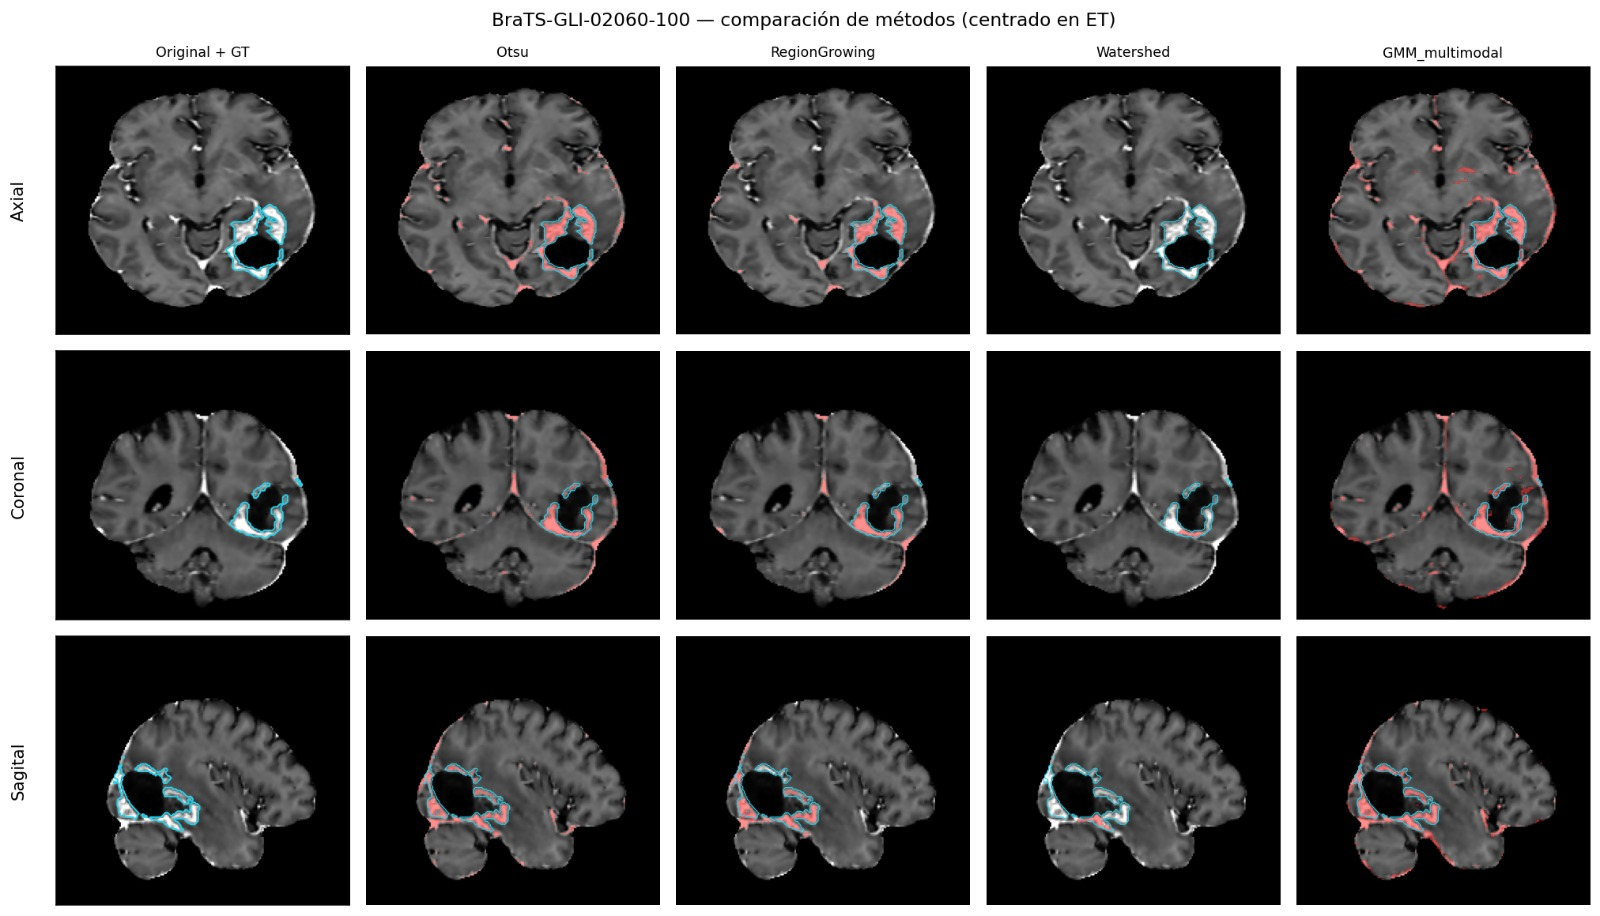
\includegraphics[width=\columnwidth]{fig2_clasicos_mosaico.png}
\caption{Comparativa de m\'{e}todos cl\'{a}sicos en tres vistas
(caso BraTS-GLI-02060-100).
El contorno cian delimita la anotaci\'{o}n y la superposici\'{o}n
roja corresponde a la predicci\'{o}n de cada m\'{e}todo.
La mezcla de gaussianas (columna derecha) sobresegmenta claramente,
capturando tejido perif\'{e}rico no tumoral.}
\label{fig:clasicos}
\end{figure}

\subsection{Mapa de sustracci\'{o}n T1c$-$T1n y FastMarching}

El gadolinio no atraviesa la barrera hematoencef\'{a}lica intacta,
por lo que el realce en T1c respecto a T1n es espec\'{i}fico del
tejido tumoral activo o de zonas de ruptura de dicha barrera.
Esta propiedad se explota mediante el mapa de sustracci\'{o}n
$S = \mathrm{clip}(T1c_n - T1n_n,\, 0,\, 1)$, donde T1c$_n$ y
T1n$_n$ se normalizan con el mismo factor m\'{a}ximo conjunto para
preservar la relaci\'{o}n de escala entre ambas modalidades.
El mapa resultante, suavizado con $\sigma = 0{,}8$, presenta valores
medios de 0,24 dentro del tumor realzante y de 0,04 en tejido sano
(Fig.~\ref{fig:mapa}), con los vasos sangu\'{i}neos en el extremo
superior ($S > 0{,}55$), excluibles por umbral.
Esta discriminaci\'{o}n no es posible con T1c aislado porque el
tejido sano brillante tambi\'{e}n lo era antes del contraste.

\begin{figure}[h]
\centering
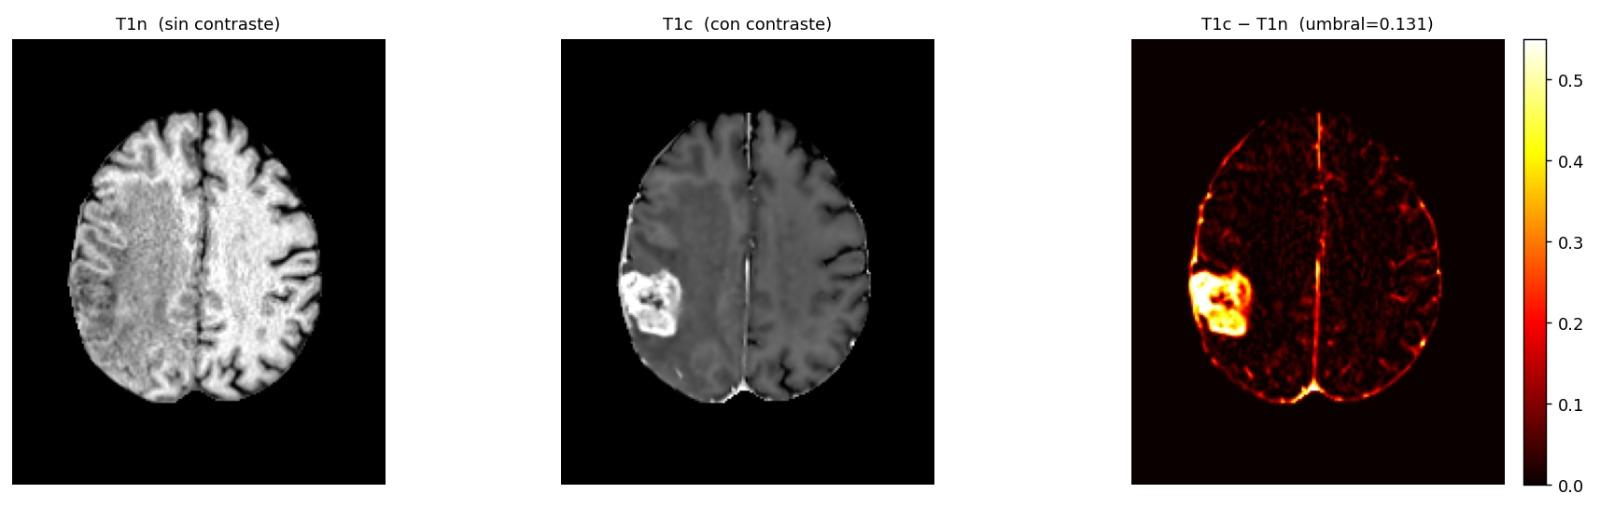
\includegraphics[width=\columnwidth]{fig1_mapa_sustraccion.jpg}
\caption{Mapa de sustracci\'{o}n T1c$-$T1n (caso
BraTS-GLI-02119-101, corte axial).
De izquierda a derecha: T1n sin contraste, T1c con contraste y
mapa de diferencia en escala de calor.
El tumor realzante aparece en amarillo-blanco, con valores
en torno a 0,24, mientras el tejido sano permanece oscuro.}
\label{fig:mapa}
\end{figure}

El algoritmo de FastMarching resuelve la ecuaci\'{o}n Eikonal
$|\nabla T(x)| \cdot S(x) = 1$ desde una semilla $x_0$ con
condici\'{o}n inicial $T(x_0) = 0$.
En las regiones de alto realce el frente avanza r\'{a}pidamente,
produciendo tiempos de llegada bajos; en tejido sano avanza lento,
produciendo tiempos altos; y en los bordes del tumor, donde el
mapa cae abruptamente, el frente se desacelera de forma natural.
La predicci\'{o}n final se obtiene umbralizando $T \leq t^* = 35$,
valor calibrado emp\'{i}ricamente.

La localizaci\'{o}n de la semilla inicial es determinante para el
resultado.
Se evaluaron tres estrategias:
una semilla autom\'{a}tica sin acceso a la anotaci\'{o}n, que
selecciona el v\'{o}xel con mayor producto
$T1c_{\text{limpio}} \times S$ excluyendo vasos, con suavizado
uniforme de tama\~{n}o~5 para robustez;
la semilla en el centroide geom\'{e}trico del tumor realzante
seg\'{u}n la anotaci\'{o}n, que representa una cota superior
te\'{o}rica del m\'{e}todo;
y una semilla aleatoria dentro de la anotaci\'{o}n, que eval\'{u}a
la robustez del algoritmo ante variaciones en la posici\'{o}n
inicial.
Los resultados se presentan en la Tabla~\ref{tab:fm} y la
Fig.~\ref{fig:fm}.

\begin{table}[h]
\centering\small
\caption{Resultados del FastMarching seg\'{u}n la estrategia de
semilla (20~casos con tumor realzante presente).
Las semillas basadas en la anotaci\'{o}n representan cotas
superiores, no m\'{e}todos completamente autom\'{a}ticos.}
\label{tab:fm}
\begin{tabular}{lccc}
\toprule
Semilla & Dice & M\'{a}x & M\'{i}n ($>0$) \\
\midrule
Autom\'{a}tica & 0,286 & 0,710 & 0,040 \\
Aleatoria en anotaci\'{o}n & 0,324 & 0,600 & 0,060 \\
\textbf{Centroide de anotaci\'{o}n} & \textbf{0,509} & \textbf{0,761} & 0,031 \\
\bottomrule
\end{tabular}
\end{table}

\begin{figure}[h]
\centering
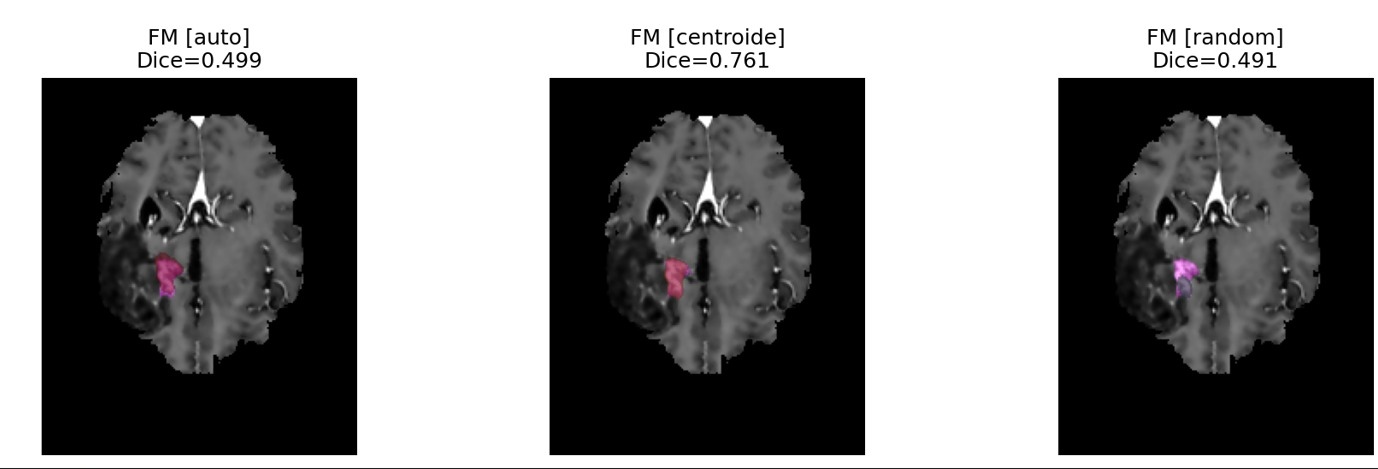
\includegraphics[width=\columnwidth]{fig3_fm_semillas.png}
\caption{FastMarching con tres estrategias de semilla sobre el
mismo caso.
La semilla centroide produce la mejor cobertura (Dice~0,761).
La brecha promedio entre la semilla autom\'{a}tica (Dice~0,286)
y la semilla centroide (Dice~0,509) sugiere que el desempe\~{n}o
del FastMarching est\'{a} fuertemente condicionado por la
localizaci\'{o}n inicial de la semilla.}
\label{fig:fm}
\end{figure}

\subsection{Contornos activos variacionales}

Los contornos activos abordan la segmentaci\'{o}n como un problema
de minimizaci\'{o}n de energ\'{i}a sobre la forma y posici\'{o}n de
un contorno deformable, lo que los hace menos sensibles a la
posici\'{o}n exacta de la semilla que el FastMarching, pues el
contorno puede corregirse iterativamente.
Se implementaron cuatro variantes, todas con una inicializaci\'{o}n
autom\'{a}tica h\'{i}brida: una mezcla de gaussianas de tres componentes
sobre T1c localiza la masa realzante ---la componente de mayor media--- y,
cuando \'{e}sta degenera por captar tejido sano brillante, se recurre al
\emph{blob} dominante del mapa de sustracci\'{o}n.
Una salvaguarda revierte a esta semilla cualquier evoluci\'{o}n que colapse,
se fugue en volumen o se desplace a otra regi\'{o}n, de modo que un contorno
degenerado nunca puntu\'{a} por debajo de la inicializaci\'{o}n.

El spline variacional de Chan--Vese~\cite{chan2001active} minimiza
la diferencia entre las medias de intensidad dentro y fuera del
contorno, expresada como
\begin{equation}
E(C,c_1,c_2) = \mu|C|
  + \lambda_1\!\int_{\mathrm{int}(C)}\!(u_0-c_1)^2\,dx
  + \lambda_2\!\int_{\mathrm{ext}(C)}\!(u_0-c_2)^2\,dx,
\end{equation}
sin depender del gradiente de la imagen, lo que lo hace robusto a
bordes difusos caracter\'{i}sticos del tumor realzante
post-quir\'{u}rgico.
La variante B-spline regulariza la frontera del resultado de
Chan--Vese reescribi\'{e}ndola corte a corte como un B-spline c\'{u}bico
peri\'{o}dico con continuidad $C^2$, lo que suaviza el dentado de la
m\'{a}scara de v\'{o}xeles sin a\~{n}adir par\'{a}metros libres.
El \textit{level set} geod\'{e}sico~\cite{caselles1997geodesic}
evoluciona una funci\'{o}n de distancia con signo guiada por
$g(x) = 1/(1 + |\nabla G_\sigma \ast u_0|^2)$, que se aproxima a
cero en los bordes fuertes de la imagen y desacelera la
propagaci\'{o}n del frente.
El snake param\'{e}trico cl\'{a}sico minimiza la energ\'{i}a
combinada de rigidez, elasticidad y fuerza imagen sobre un contorno
discretizado.

La Fig.~\ref{fig:todos} compara todos los m\'{e}todos del trabajo
sobre un caso representativo.
Los resultados cuantitativos de los contornos activos se muestran
en la Tabla~\ref{tab:contornos}.

\begin{figure*}[t]
\centering
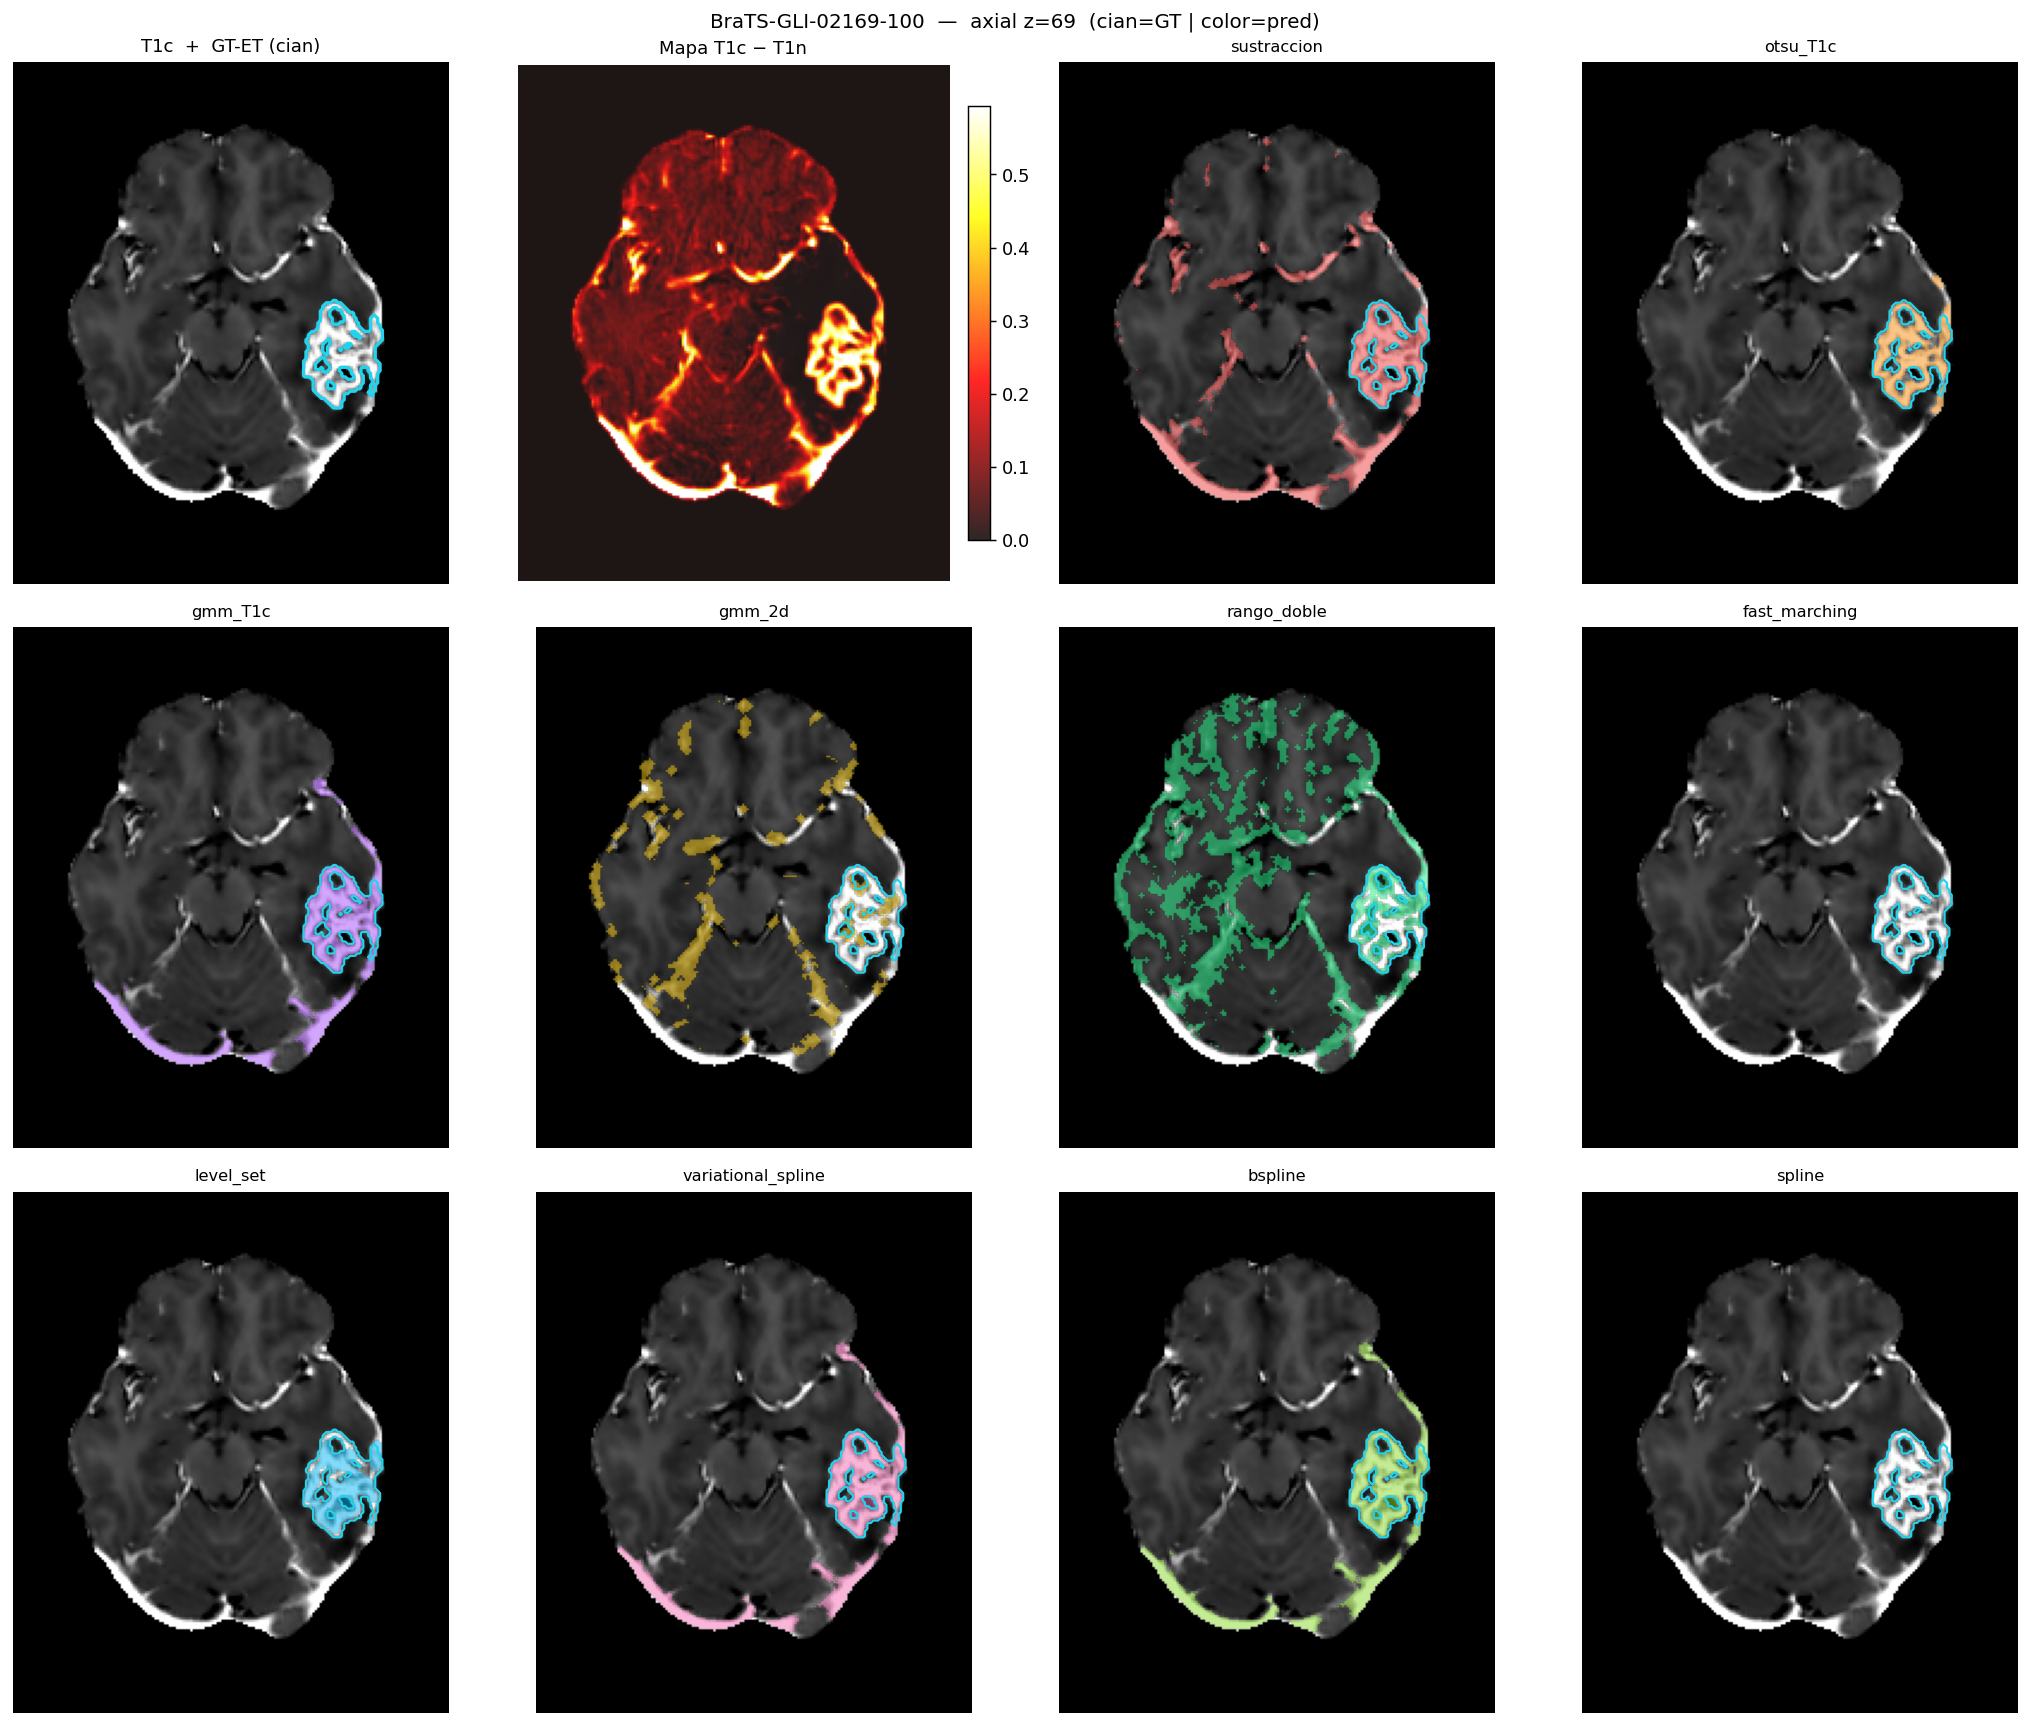
\includegraphics[width=\textwidth]{fig4_todos_metodos.png}
\caption{Comparativa de todos los m\'{e}todos del trabajo
(caso BraTS-GLI-02169-100, corte axial $z = 69$).
El contorno cian delimita la anotaci\'{o}n de referencia y el
color de relleno corresponde a la predicci\'{o}n de cada
m\'{e}todo.
Los contornos activos variacionales (fila inferior) logran la
mejor correspondencia con la anotaci\'{o}n, seguidos del
FastMarching.
Los m\'{e}todos de intensidad pura (filas superiores) presentan
sobresegmentaci\'{o}n o subsegmentaci\'{o}n sistem\'{a}tica.}
\label{fig:todos}
\end{figure*}

\begin{table}[h]
\centering\small
\caption{Resultados de los contornos activos y del FastMarching
(20~casos). La columna ``$>$0,75'' indica cu\'{a}ntos casos
superan ese Dice. Los resultados son indicativos dado el tama\~{n}o
de la muestra.}
\label{tab:contornos}
\begin{tabular}{lcccc}
\toprule
M\'{e}todo & Dice & Mediana & M\'{a}x & $>0{,}75$ \\
\midrule
\textbf{Spline var.\ Chan--Vese} & \textbf{0,505} & 0,506 & 0,860 & 5 \\
B-spline & 0,473 & 0,465 & 0,794 & 2 \\
Level set geod. & 0,455 & 0,475 & 0,781 & 2 \\
Snake param. & 0,450 & 0,484 & 0,795 & 2 \\
\midrule
FM centroide (cota sup.) & 0,509 & --- & 0,761 & --- \\
FM autom\'{a}tica & 0,286 & --- & 0,710 & --- \\
\bottomrule
\end{tabular}
\end{table}

% ═══════════════════════════════════════════
\section{Visualizaci\'{o}n 3D}
% ═══════════════════════════════════════════

Para facilitar la inspecci\'{o}n visual, se generaron mallas
tridimensionales de la predicci\'{o}n y la anotaci\'{o}n mediante el
algoritmo \textit{marching cubes}~\cite{lorensen1987marching},
aplicando el espaciado f\'{i}sico real de los v\'{o}xeles y un
suavizado de Taubin.
Para la comparaci\'{o}n visual de superficies, las mallas de la
predicci\'{o}n y la anotaci\'{o}n se reconstruyen adem\'{a}s mediante
reconstrucci\'{o}n de Poisson \emph{screened}~\cite{kazhdan2013screened}
a partir de su nube de puntos orientada, obteniendo superficies suaves y
cerradas.
Las mallas se exportan en formato PLY y se integran en un visor
web interactivo basado en Three.js que permite superponer ambas
mallas con control de opacidad y alternar entre vista 2D y 3D.
La validaci\'{o}n de escala confirma que el volumen de la malla de
referencia reproduce el calculado en el an\'{a}lisis exploratorio
con un error relativo inferior al 5\% en 7 de los 8~casos
evaluados, lo que garantiza la consistencia geom\'{e}trica del
pipeline.

La Fig.~\ref{fig:3d} muestra el caso con mayor Dice del trabajo,
el caso~02108-100 segmentado con el spline variacional
Chan--Vese, con un Dice de 0,860.
La mayor parte del volumen tumoral se captura correctamente; los
falsos positivos visibles en rojo coinciden con zonas perilesionales
de alta intensidad en T1c que el mapa de sustracci\'{o}n no
discrimina completamente.

\begin{figure}[h]
\centering
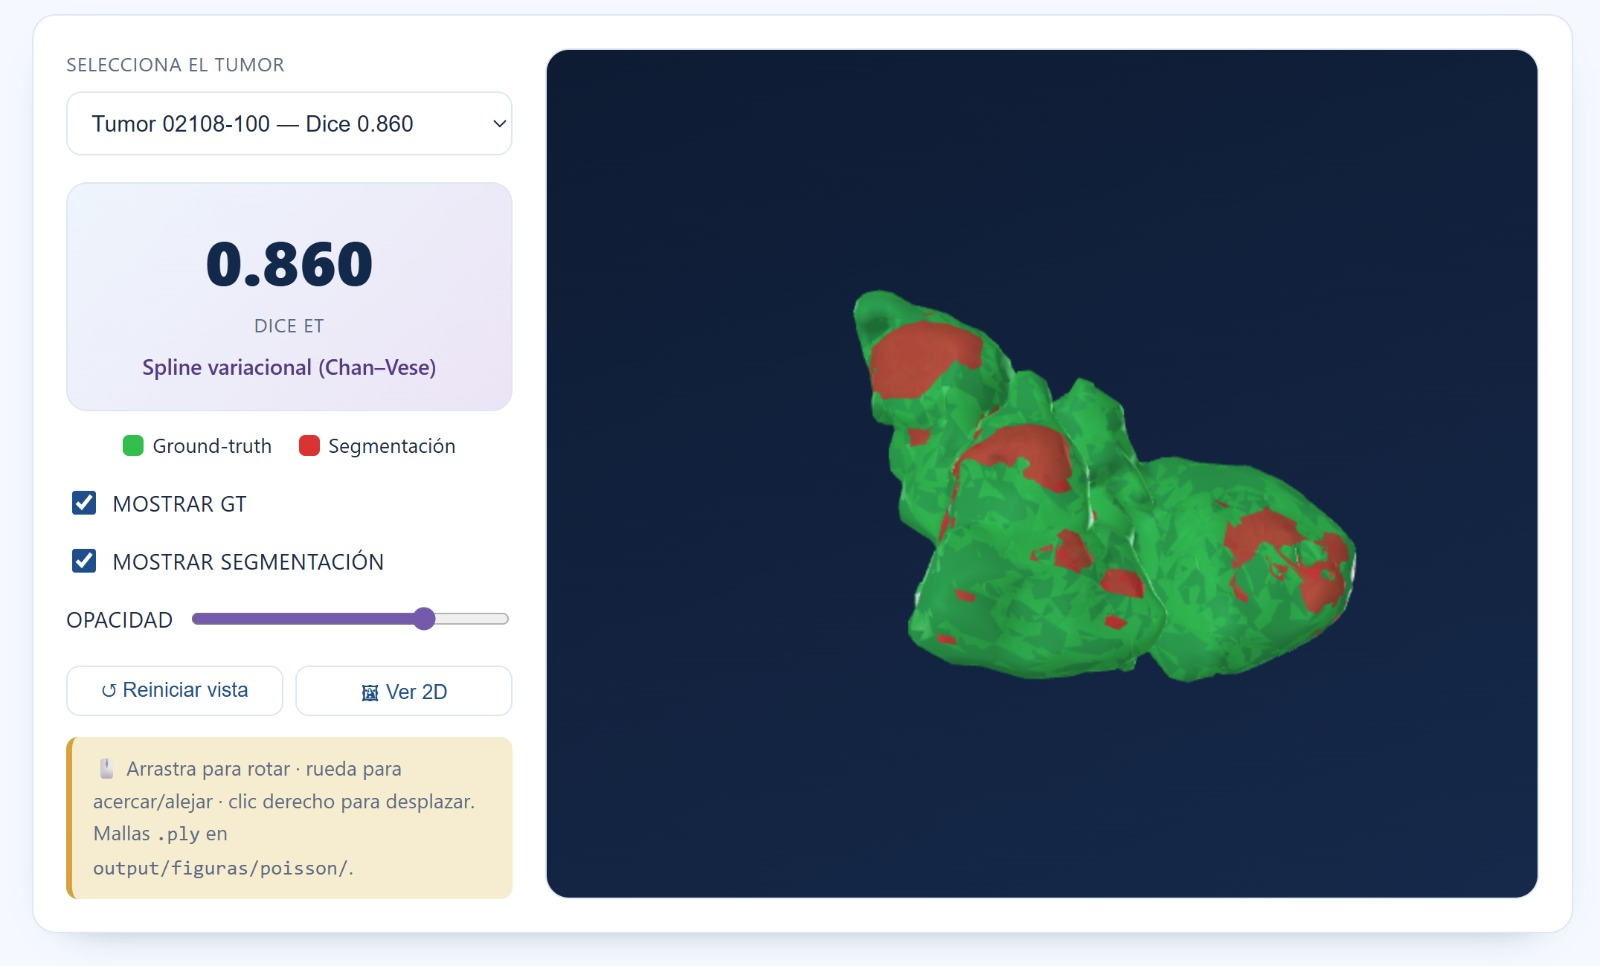
\includegraphics[width=0.92\columnwidth]{fig5_visor3d.png}
\caption{Visor 3D interactivo: anotaci\'{o}n de referencia en verde
y predicci\'{o}n del spline variacional Chan--Vese en rojo.
Caso~02108-100, Dice~0,860.
Las zonas verdes sin rojo corresponden a falsos negativos y las
rojas sin verde a falsos positivos.}
\label{fig:3d}
\end{figure}

% ═══════════════════════════════════════════
\section{Resultados y discusi\'{o}n}
% ═══════════════════════════════════════════

La Tabla~\ref{tab:global} presenta todos los m\'{e}todos ordenados
por Dice medio.
El an\'{a}lisis permite identificar tres reg\'{i}menes de
desempe\~{n}o diferenciados.

Los m\'{e}todos de intensidad pura sobre T1c quedan limitados a un
rango de Dice entre 0,09 y 0,37.
El an\'{a}lisis de ablaci\'{o}n confirm\'{o} que este techo es
estructural: aun con la entrada m\'{a}s separable posible
(FDR~1,80), el Dice del mejor ensamble se estanca en 0,370.
La raz\'{o}n es geom\'{e}trica: el histograma de T1c es unimodal
en la mayor\'{i}a de los casos post-tratamiento, de modo que el
umbral alto de Otsu cae en un punto arbitrario que mezcla realce
con tejido sano brillante.
El crecimiento de regiones y el \textit{watershed} pueden
localizarse correctamente cuando la semilla est\'{a} bien ubicada,
pero la heterogeneidad del anillo post-quir\'{u}rgico limita su
expansi\'{o}n.
La mezcla de gaussianas multimodal ilustra que incorporar T2w y
T2-FLAIR sin un modelo de forma empeora el resultado: captura un
c\'{u}mulo amplio dominado por el edema, con alta sensibilidad
pero Dice de 0,094.

El mapa de sustracci\'{o}n T1c$-$T1n cambia cualitativamente este
panorama.
Todos los m\'{e}todos que incorporan esta se\~{n}al superan o igualan
el mejor m\'{e}todo de intensidad pura.
El motivo es que la diferencia T1c$-$T1n es espec\'{i}fica del
gadolinio: el tejido sano brillante en T1c tambi\'{e}n lo era en
T1n, de modo que su diferencia es cercana a cero, mientras que el
tumor realzante acumula contraste y produce una diferencia alta.

Entre los m\'{e}todos avanzados, el spline variacional Chan--Vese
y el FastMarching con semilla centroide son comparables en Dice
medio (0,505 y 0,509 respectivamente), pero difieren en robustez.
El FastMarching con semilla autom\'{a}tica baja a 0,286 cuando la
semilla cae en tejido perilesional o en un vaso sangu\'{i}neo,
porque la propagaci\'{o}n unidireccional no puede corregirse.
Los contornos activos, al minimizar una energ\'{i}a global de forma
iterativa, son m\'{a}s tolerantes a variaciones en la semilla:
el spline variacional mantiene Dice~0,505 con semilla
autom\'{a}tica.

En t\'{e}rminos de comparaci\'{o}n con la literatura, los mejores
m\'{e}todos cl\'{a}sicos quedan aproximadamente 0,35 puntos de Dice
por debajo de nnU-Net~\cite{baig2024nnunet} en promedio.
No obstante, algunos casos individuales alcanzan Dice altos, como
0,860 con el spline variacional, lo que muestra que el enfoque
puede ser competitivo en casos con tumor realzante bien definido,
aunque estos resultados son indicativos dado el tama\~{n}o de la
muestra de 20~casos.

\begin{table}[h]
\centering\small
\caption{Comparaci\'{o}n global de todos los m\'{e}todos
(20~casos). \colorbox{cellmid}{Amarillo}: Dice $\ge 0{,}40$.
\colorbox{cellbad}{Rojo}: Dice $< 0{,}40$.
Los m\'{e}todos con semilla de cota superior no son completamente
autom\'{a}ticos.}
\label{tab:global}
\begin{tabular}{lcc}
\toprule
M\'{e}todo & Dice & M\'{a}x \\
\midrule
\cm{FM centroide (cota sup.)} & \cm{0,509} & 0,761 \\
\cm{Spline var.\ Chan--Vese} & \cm{0,505} & 0,860 \\
\cm{B-spline} & \cm{0,473} & 0,794 \\
\cm{Level set geod.} & \cm{0,455} & 0,781 \\
\cm{Snake param.} & \cm{0,450} & 0,795 \\
\cm{Sustracci\'{o}n T1c$-$T1n} & \cm{0,447} & 0,792 \\
\cb{GMM 2D} & \cb{0,374} & 0,828 \\
\cb{Uni\'{o}n+post (ensamble)} & \cb{0,370} & --- \\
\cb{FM autom\'{a}tica} & \cb{0,286} & 0,710 \\
\cb{Rango doble} & \cb{0,238} & 0,589 \\
\cb{Otsu base} & \cb{0,164} & --- \\
\cb{GMM multimodal} & \cb{0,094} & --- \\
\bottomrule
\end{tabular}
\end{table}

En cuanto a las limitaciones, el estudio se basa en 20~casos
aleatorios y las cifras son indicativas; estudios futuros
deber\'{a}n validarlas sobre muestras m\'{a}s amplias e incluso
reportar desviaciones est\'{a}ndar.
El registro se evalu\'{o} sobre una perturbaci\'{o}n r\'{i}gida
conocida y no generaliza directamente a deformaciones no
r\'{i}gidas en escenarios longitudinales.
La semilla autom\'{a}tica del FastMarching falla cuando el
v\'{o}xel de mayor score coincide con un vaso sangu\'{i}neo o con
tejido perilesional de alta intensidad en T1c.

% ═══════════════════════════════════════════
\section{Conclusiones}
% ═══════════════════════════════════════════

Este trabajo cuantifica emp\'{i}ricamente los alcances y
l\'{i}mites de los m\'{e}todos cl\'{a}sicos para la segmentaci\'{o}n
del tumor realzante en BraTS~2024 GLI post-tratamiento.
El hallazgo m\'{a}s importante es que los m\'{e}todos de intensidad
pura sobre T1c presentan un techo estructural de Dice en torno
a 0,37, impuesto por la forma del tumor realzante post-quir\'{u}rgico
y no por el preprocesamiento, cuyo an\'{a}lisis de ablaci\'{o}n
muestra que mejora la separabilidad de forma sistem\'{a}tica.
El mapa de sustracci\'{o}n T1c$-$T1n rompe ese techo al proporcionar
una se\~{n}al espec\'{i}fica del gadolinio que distingue el realce
tumoral del tejido sano brillante.
Tanto el algoritmo de FastMarching como los contornos activos
variacionales, guiados por dicho mapa, superan Dice~0,50 con
semilla centroide o con semilla autom\'{a}tica respectivamente.
El spline variacional Chan--Vese emerge como el mejor m\'{e}todo
del trabajo con un Dice medio de 0,505 y un m\'{a}ximo individual
de 0,860, siendo adem\'{a}s el m\'{a}s robusto a la posici\'{o}n
de la semilla gracias a su formulaci\'{o}n variacional.

La brecha entre la semilla autom\'{a}tica y la semilla centroide
en el FastMarching (0,286 frente a 0,509) se\~{n}ala la
localizaci\'{o}n de la semilla como la principal l\'{i}nea de mejora:
reemplazar la heur\'{i}stica actual por un detector de punto
liviano podr\'{i}a elevar el desempe\~{n}o autom\'{a}tico al nivel
de la cota superior sin modificar el resto del pipeline.
Adicionalmente, el pipeline de preprocesamiento y el mapa de
sustracci\'{o}n son directamente reutilizables como etapa de
entrada para modelos de aprendizaje profundo, lo que constituye
una contribuci\'{o}n modular con valor independiente.

\begin{thebibliography}{99}

\bibitem{louis2021who}
D.~N.~Louis \emph{et al.},
``The 2021 WHO Classification of Tumors of the Central Nervous
System: a summary,''
\emph{Neuro-Oncology}, vol.~23, no.~8, pp.~1231--1251, 2021.

\bibitem{mesfin2024gliomas}
F.~B.~Mesfin and M.~A.~Al-Dhahir,
``Gliomas,''
in \emph{StatPearls}, StatPearls Publishing, 2024.

\bibitem{bhattacharya2024posttreatment}
D.~Bhattacharya \emph{et al.},
``Imaging assessment of post-treatment gliomas: a review,''
\emph{Clinical Radiology}, vol.~79, no.~3, pp.~e376--e392, 2024.

\bibitem{visser2019interobserver}
M.~Visser \emph{et al.},
``Inter-rater agreement in glioma segmentations on longitudinal
MRI,''
\emph{NeuroImage: Clinical}, vol.~22, art.~101727, 2019.

\bibitem{deverdier2024brats}
M.~Correia~de~Verdier \emph{et al.},
``The 2024 Brain Tumor Segmentation (BraTS) Challenge: Glioma
Segmentation on Post-treatment MRI,''
\emph{arXiv:2405.18368}, 2024.

\bibitem{lloyd2010itk}
B.~C.~Lowekamp, D.~T.~Chen, L.~Ib\'{a}\~{n}ez and D.~Blezek,
``The design of SimpleITK,''
\emph{Frontiers in Neuroinformatics}, vol.~7, p.~45, 2013.

\bibitem{gyorfi2021ensemble}
\'A.~Gy\H{o}rfi, L.~Szil\'{a}gyi and L.~Kov\'{a}cs,
``A fully automatic procedure for brain tumor segmentation from
multi-spectral MRI records using ensemble learning and atlas-based
data enhancement,''
\emph{Applied Sciences}, vol.~11, no.~2, art.~564, 2021.

\bibitem{baig2024nnunet}
S.~Baig \emph{et al.},
``Segmentation of pre- and posttreatment diffuse glioma tissue
subregions including resection cavities,''
\emph{Neuro-Oncology Advances}, vol.~6, no.~1, art.~vdae140,
2024.

\bibitem{luque2024extension}
A.~Bj{\o}rnerud \emph{et al.},
``Standardized evaluation of the extent of resection in
glioblastoma with automated early post-operative segmentation,''
\emph{Frontiers in Radiology}, vol.~4, art.~1357341, 2024.

\bibitem{tustison2010n4}
N.~J.~Tustison \emph{et al.},
``N4ITK: Improved N3 bias correction,''
\emph{IEEE Trans.\ Med.\ Imag.}, vol.~29, no.~6,
pp.~1310--1320, 2010.

\bibitem{mattes2003}
D.~Mattes, D.~R.~Haynor, H.~Vesselle, T.~K.~Lewellyn and
W.~Eubank,
``PET-CT image registration in the chest using free-form
deformations,''
\emph{IEEE Trans.\ Med.\ Imag.}, vol.~22, no.~1,
pp.~120--128, 2003.

\bibitem{otsu1979}
N.~Otsu,
``A threshold selection method from gray-level histograms,''
\emph{IEEE Trans.\ Syst., Man, Cybern.}, vol.~9, no.~1,
pp.~62--66, 1979.

\bibitem{vincent1991watersheds}
L.~Vincent and P.~Soille,
``Watersheds in digital spaces: an efficient algorithm based on
immersion simulations,''
\emph{IEEE Trans.\ Pattern Anal.\ Mach.\ Intell.}, vol.~13,
no.~6, pp.~583--598, 1991.

\bibitem{pedregosa2011scikit}
F.~Pedregosa \emph{et al.},
``Scikit-learn: Machine learning in Python,''
\emph{J.\ Mach.\ Learn.\ Res.}, vol.~12, pp.~2825--2830, 2011.

\bibitem{chan2001active}
T.~F.~Chan and L.~A.~Vese,
``Active contours without edges,''
\emph{IEEE Trans.\ Image Process.}, vol.~10, no.~2,
pp.~266--277, 2001.

\bibitem{caselles1997geodesic}
V.~Caselles, R.~Kimmel and G.~Sapiro,
``Geodesic active contours,''
\emph{Int.\ J.\ Computer Vision}, vol.~22, no.~1,
pp.~61--79, 1997.

\bibitem{lorensen1987marching}
W.~E.~Lorensen and H.~E.~Cline,
``Marching cubes: A high resolution 3D surface construction
algorithm,''
\emph{ACM SIGGRAPH}, vol.~21, no.~4, pp.~163--169, 1987.

\bibitem{kazhdan2013screened}
M.~Kazhdan and H.~Hoppe,
``Screened Poisson surface reconstruction,''
\emph{ACM Trans.\ Graphics}, vol.~32, no.~3, art.~29, 2013.

\end{thebibliography}

\end{document}
